


\subsubsection{GDN Hybrid Architecture}
\label{sec:gdn-hybrid}


\begin{figure}[H]
\centering
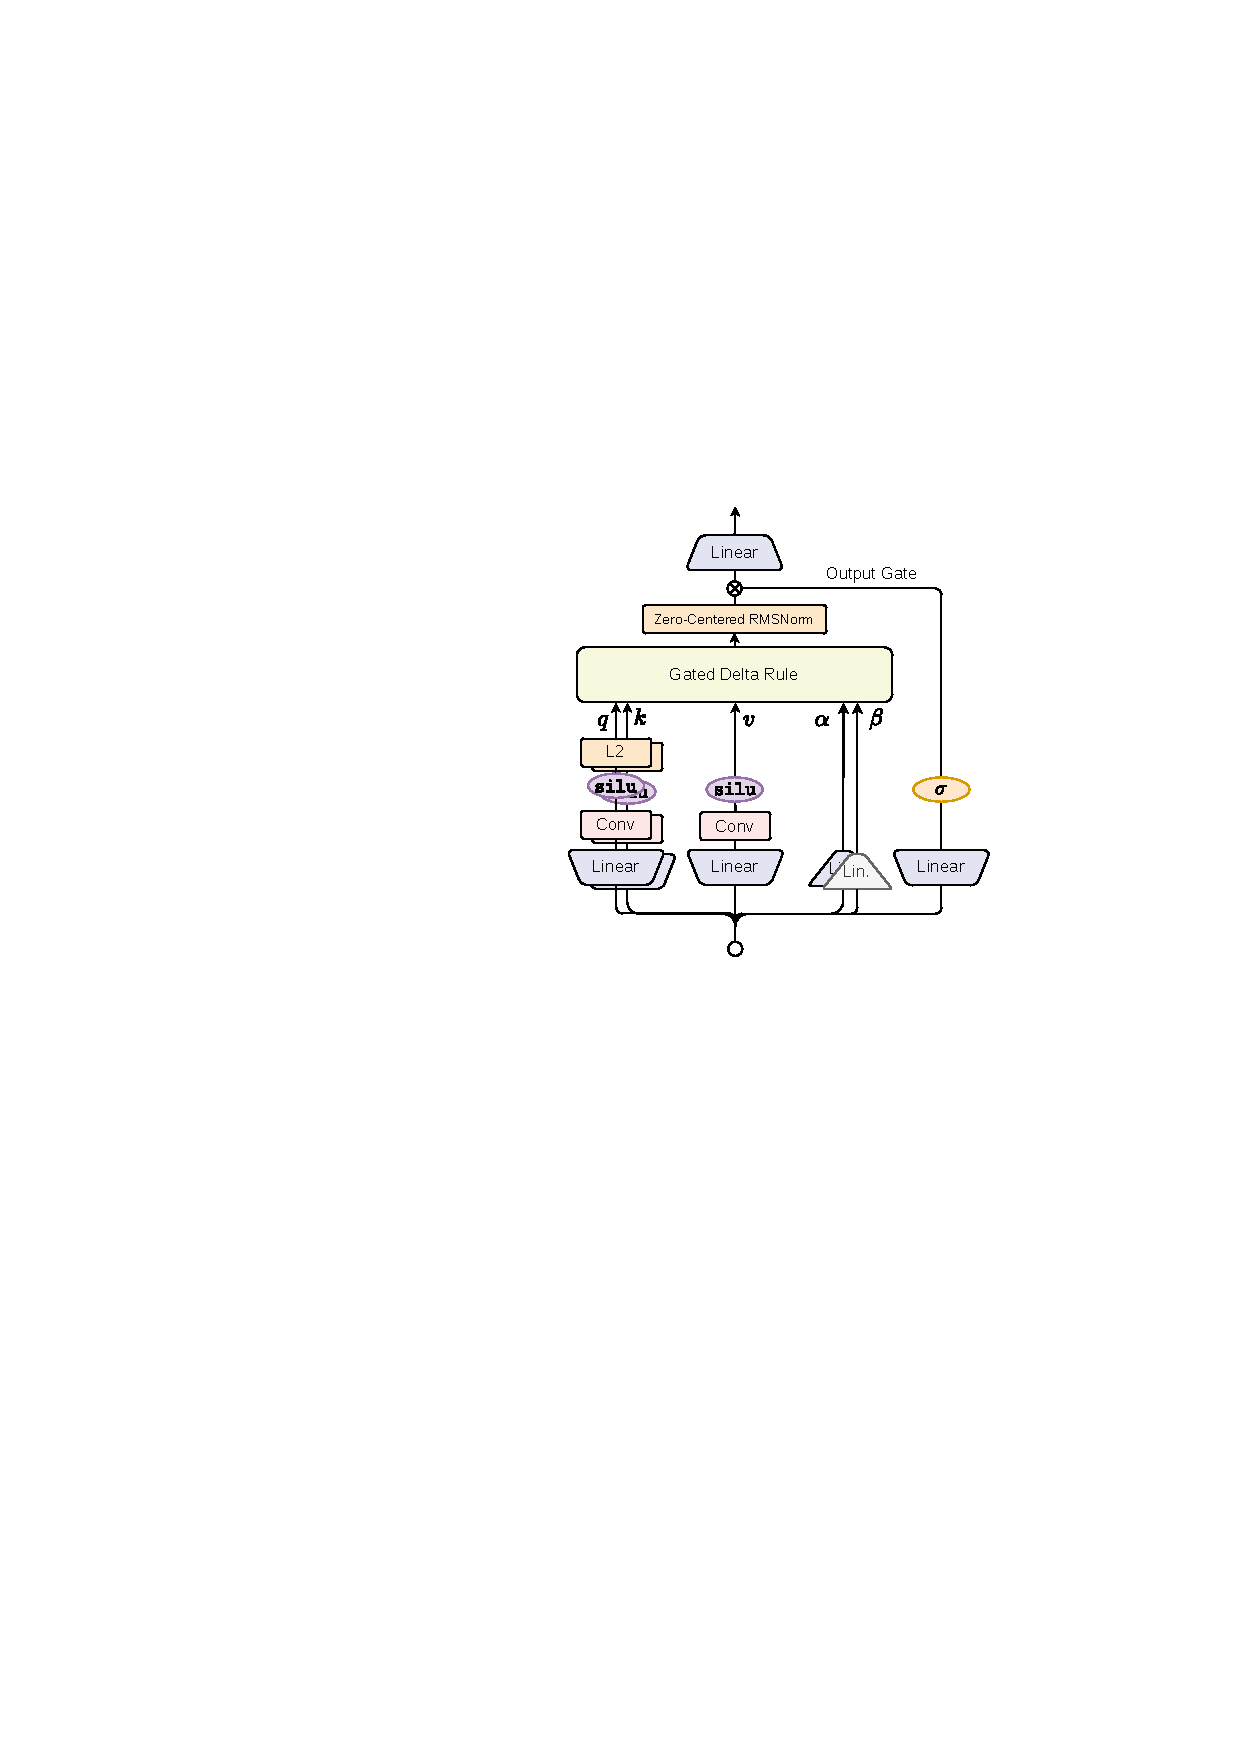
\includegraphics[pagebox=cropbox,width=0.52\linewidth]{figs/Qwen4Exp_GDN.drawio.pdf}
\caption{The Gated DeltaNet token mixer. The projected query, key, and value streams pass through short causal convolutions; queries and keys are L2-normalized before the gated delta recurrence. The decay gate $\alpha_t$ and write gate $\beta_t$ control the recurrent update, while a sigmoid output gate modulates the zero-centered RMS-normalized output.}
\label{fig:gdn-module}
\end{figure}

\paragraph{Motivation.}
\label{sec:gdn-motivation}

Full self-attention provides direct content-based access to every preceding token, but its token-mixing cost grows quadratically with sequence length and its key--value (KV) cache grows linearly during autoregressive generation~\citep{vaswani2017attention}. Sliding-window attention (SWA) replaces global access with a bounded local receptive field, reducing both computation and cache consumption. However, information outside the window can only propagate indirectly through depth. This creates a tension between efficient local processing and persistent content-dependent memory.

We address this tension with a layer-wise hybrid of Gated DeltaNet (GDN)~\citep{yang2024gated} and global attention. GDN compresses the prefix into a fixed-size recurrent state and updates that state according to the current content, while the interleaved global-attention layers retain direct token-level retrieval that is difficult for any finite-state recurrent memory to reproduce exactly.


This design choice is consistent with the architecture ablation reported in Tab.~\ref{tab:gdn-main-results}. Relative to the full-attention Transformer baseline, the GDN-hybrid model improves 8 of the 9 selected benchmarks. Relative to the SWA-hybrid, it is stronger on seven of the nine benchmarks. These results motivate a hybrid design, but they do not by themselves isolate which architectural component causes each improvement.

\paragraph{Gated Delta Recurrence.}
\label{sec:gdn-recurrence}

Linear attention can be interpreted as a fast-weight memory that stores key--value associations in a matrix state~\citep{schlag2021linear}. For each head, let $\bm{q}_t,\bm{k}_t\in\mathbb{R}^{d_k}$ and $\bm{v}_t\in\mathbb{R}^{d_v}$. Following the implementation convention, GDN maintains a state $\bm{S}_t\in\mathbb{R}^{d_k\times d_v}$, which is the transpose of the state convention used in the original formulation, and applies the gated delta rule~\citep{yang2024gated}:
\begin{align}
\widetilde{\bm{S}}_{t-1} &= \alpha_t \bm{S}_{t-1}, \\
\bm{e}_t &= \bm{v}_t - \widetilde{\bm{S}}_{t-1}^{\top}\bm{k}_t, \\
\bm{S}_t &= \widetilde{\bm{S}}_{t-1}
    + \beta_t\bm{k}_t\bm{e}_t^{\top}, \\
\bm{y}_t &= \bm{S}_t^{\top}\bm{q}_t,
\end{align}
where $\alpha_t\in(0,1)$ is a data-dependent decay and $\beta_t\in(0,1)$ controls the delta update. Equivalently,
\begin{equation}
\bm{S}_t
= \alpha_t\left(\bm{I}-\beta_t\bm{k}_t\bm{k}_t^{\top}\right)\bm{S}_{t-1}
+ \beta_t\bm{k}_t\bm{v}_t^{\top}.
\end{equation}

The two gates play complementary roles. The decay $\alpha_t$ globally controls the lifetime of the existing state, whereas the delta term first estimates the value already associated with $\bm{k}_t$ and writes only the residual error. Consequently, repeated or similar keys update an existing association instead of accumulating unbounded outer products. This targeted erase-and-write operation distinguishes GDN from purely additive linear attention.

\paragraph{GDN Parameterization.}
\label{sec:gdn-parameterization}

Given the normalized residual-stream input $\bm{x}_t\in\mathbb{R}^{d}$, GDN computes content features using learned projections followed by a short depthwise causal convolution:
\begin{align}
\bm{q}_t &= \operatorname{L2Norm}\left(\operatorname{SiLU}\left(\operatorname{ShortConv}(\bm{W}_q\bm{x}_t)\right)\right), \\
\bm{k}_t &= \operatorname{L2Norm}\left(\operatorname{SiLU}\left(\operatorname{ShortConv}(\bm{W}_k\bm{x}_t)\right)\right), \\
\bm{v}_t &= \operatorname{SiLU}\left(\operatorname{ShortConv}(\bm{W}_v\bm{x}_t)\right).
\end{align}
Short convolution supplies an explicit local inductive bias before information is compressed into the recurrent state. L2 normalization bounds the magnitudes of $\bm{q}$/$\bm{k}$ and stabilizes the rank-one delta transition.

The write strength and decay are parameterized as
\begin{align}
\beta_t &= \sigma(\bm{W}_{\beta}\bm{x}_t), \\
\alpha_t &= \exp\left[-\exp(\bm{A})
    \operatorname{softplus}(\bm{W}_{\alpha}\bm{x}_t+\bm{b}_{\alpha})\right].
\end{align}
After applying the recurrence independently across heads, the head outputs are normalized and modulated by an input-dependent output gate:
\begin{equation}
\label{eq:gdn-output-gate}
\bm{o}_t = \bm{W}_o\left[
\sigma(\bm{W}_z\bm{x}_t)
\odot \operatorname{RMSNorm}(\bm{y}_t)
\right].
\end{equation}
Unlike the original GDN, which uses a SiLU output gate, we use the bounded sigmoid gate in Equation~\eqref{eq:gdn-output-gate} and observe consistent improvements across our experiments. 
Following Qwen3-Next, we adopt zero-centered RMSNorm to constrain the growth of RMSNorm weights. The same formulation is consistently applied to all other RMSNorm layers used throughout the model.
Figure~\ref{fig:gdn-module} summarizes the complete GDN token-mixing path.

At the model level, our hybrid architecture retains rotary position embeddings (RoPE)~\citep{rope} in its full-attention layers. 
RoPE and a NoPE variant without positional encoding show little difference during pretraining, but \textit{the NoPE variant exhibits a substantially higher rate of endless generation after post-training and is therefore more likely to fail to terminate.}
We place one such full-attention layer in every four layers, with the other three layers using GDN. This schedule strikes a favorable balance between efficiency and quality, while periodic full attention is particularly important for long-context performance.

\paragraph{Kernel Efficiency.}
\label{sec:gdn-efficiency}

For efficiency, we optimize the GDN kernel with FlashQLA, a TileLang-based fused linear-attention kernel library. Across multiple settings on NVIDIA GPUs, FlashQLA achieves a $2$--$3\times$ forward speedup and an approximately $2\times$ backward speedup over the FLA Triton kernel~\citep{yang2024fla}. The implementation and benchmarks are available at \url{https://github.com/QwenLM/FlashQLA}.

\paragraph{Architecture Ablation.}
\label{sec:gdn-ablation}

We compare three checkpoints evaluated by the same evaluation pipeline: a full-attention Transformer, an SWA hybrid, and the GDN hybrid. Both hybrid variants use one full-attention layer in every four layers; the remaining token-mixing layers use SWA or GDN, respectively, with a window size of 128 for the SWA layers. Each checkpoint corresponds to a 28-layer 25B-A3B MoE model based on the Qwen3.5 architecture, pretrained first on 400B tokens with a 4K context length, and subsequently on 80B tokens with a 32K context length. We report knowledge results on MMLU~\citep{mmlu}, MMLU-Pro~\citep{wang2024mmlu}, and SuperGPQA~\citep{supergpqa}; STEM results on MATH~\citep{hendrycks2021measuring} and GSM8K~\citep{cobbe2021training}; reasoning results on BBH~\citep{suzgun2022bbh}; multilingual results on MMMLU~\citep{openai2024mmmlu}; and code results on EvalPlus and on MultiPL-E~\citep{cassano2023multipl}. The results are reported in Table~\ref{tab:gdn-main-results}.

\begin{table*}[t]
\centering
\small
\setlength{\tabcolsep}{3.5pt}
\caption{Architecture comparison. All values are percentages and higher is better. EvalPlus and MultiPL-E are reported with pass@1-style aggregate fields. Avg. is the unweighted arithmetic mean across the nine benchmarks. Bold denotes the best result in each column.}
\label{tab:gdn-main-results}
\resizebox{\textwidth}{!}{%
\begin{tabular}{lrrrrrrrrrr}
\toprule
& \multicolumn{3}{c}{Knowledge} & \multicolumn{2}{c}{STEM} & Reasoning & Multilingual & \multicolumn{2}{c}{Code} & \\
\cmidrule(lr){2-4} \cmidrule(lr){5-6} \cmidrule(lr){7-7} \cmidrule(lr){8-8} \cmidrule(lr){9-10}
Architecture & MMLU & MMLU-Pro & SuperGPQA & MATH & GSM8K & BBH & MMMLU & EvalPlus & MultiPL-E & Avg. \\
\midrule
Full attention
& 62.65 & 37.59 & 21.76 & 49.40 & 75.13 & 63.78 & 47.74 & 51.01 & 39.73 & 49.87 \\
SWA hybrid
& \textbf{66.30} & 40.67 & 22.45 & 45.48 & 74.22 & 65.88 & 51.33 & \textbf{52.12} & 41.93 & 51.15 \\
GDN hybrid
& 66.26 & \textbf{42.82} & \textbf{23.45} & \textbf{53.98} & \textbf{77.07} & \textbf{68.72} & \textbf{54.83} & 49.71 & \textbf{47.48} & \textbf{53.81} \\
\bottomrule
\end{tabular}
}
\end{table*}

The GDN hybrid improves over the Transformer on eight of the nine selected benchmarks and exceeds the SWA hybrid on seven. It achieves the best result on seven benchmarks and the highest overall average, while the SWA hybrid is marginally higher on MMLU and stronger on EvalPlus.
